\chapter{Introduction}
\label{sec:intro}
The problem of equivalence checking between a functional specification and an
implementation written in a low level imperative language such as C
has been of major research interest.
On one side, the functional programming model closely resembles mathematical functions,
which allows for comparatively easier verification of algorithmic correctness.
On the other hand, a low level imperative language such as C trades the safer abstractions of a functional
language for proximity to the machine language resulting in (usually) significantly faster executables, albeit at the cost of
a substantially higher possibility of algorithmic errors.
Being able to establish equivalence between the two abstractions would allow the user
to take advantage of both worlds -- (a) easier proof of functional correctness and
(b) more efficient executables.
The applications of such an equivalence checker would include (a) program verification, where
the equivalence checker is used to verify that the C implementation
behaves according to the specification and (b) translation validation, where
the equivalence checker attempts to generate a proof of equivalence across
the transformations (and translations) performed by an optimizing compiler.

The verification of a C implementation against its manually written
functional specification through manually-coded refinement proofs has been
performed extensively in the seL4 microkernel \cite{seL4}.
Frameworks for program equivalence proofs have been developed in interactive
theorem provers like Coq \cite{programEquivalenceInCoq} where correlations and invariants
are manually identified during proof codification.
On the other hand, programming languages like Dafny \cite{dafny} offer automated program
reasoning for imperative languages with abstract data types such as sets and arrays.
Such languages perform automatic compile-time checks for manually-specified
correctness predicates through SMT solvers.
Additionally, there exists significant prior work on translation validation
\cite{tvi,tristan_tv_eqsat11,stepp_eqsat_llvm11,eqsat,pec,zuck03,zuck05,heffter05,covac,c_to_verilog,kanade09,lopes16,tvoc_cav05,ddec,semalign,oopsla20,tv_oskernel,namjoshi13}
across multiple programming languages with similar models of computation.
In most of these applications, soundness is critial,
i.e., if the equivalence checker determines the programs to be equivalent, then the programs are indeed equivalent
and evidently have equivalent runtime observable behaviour. On the other hand, a sound equivalence checker may be incomplete
and fail to prove equivalence of a program pair, even if they were equivalent.

In this work, we present \toolName{}, a {\em sound} algorithm to automatically search
for a proof of equivalence between a functional specification and its
optimized C implementations. We will demonstrate how \toolName{} is capable of
proving equivalence of multiple equivalent C implementations with vastly
different (a) data layouts (e.g. array, linked list representations for a {\em list})
and (b) algorithmic strategies (e.g. alternate algorithms, optimizations) against
a {\em single} functional specification.
This opens the possibility of regression verification \cite{strichman_regressverify,felsing14},
where \toolName{} can be used to automate verification across
software updates that change memory layouts of data structures.
\vspace{-5px}
\section{A Motivating Example}
\label{sec:motivatingexample}
\vspace{-5px}
We start by restricting our attention to programs that construct, read, and write
to recursive data structures. In languages like C, pointer and array based
implementations of these data-structures are prone to safety and liveness bugs.
Similar recursive data structures are also available in safer functional languages like Haskell \cite{marlow2010haskell},
where algebraic data types (ADTs) \cite{algebraicdatatypes} ensure several safety properties.
We define a minimal functional language, called \SpecL{}, that enables the safe
and succinct specification of programs manipulating and traversing recursive data structures.
\SpecL{} is equipped with ADTs as well as boolean (\type{bool}) and fixed-width bitvector (\type{i<N>}) types.

We motivate our work by considering example \SpecL{} and C programs.
The major hurdles of our approach are listed alongside an informal discussion of our proposed solutions.
We state our primary contributions in \cref{sec:contribs} and finish with the organization of the rest of the thesis in \cref{sec:outline}.
\begin{figure}
\begin{tabular}{@{}c@{}c@{}}
\begin{subfigure}[b]{\textwidth}
\begin{center}
\begin{allLangEnvFoot}
~{\scriptsize \textcolor{mygray}{A0:}}~ type List = LNil | LCons (val:i32, tail:List).
~{\scriptsize \textcolor{mygray}{A1:}}~
~{\scriptsize \textcolor{mygray}{A2:}}~ fn mk_list_impl (n:i32) (i:i32) (l:List) : List =
~{\scriptsize \textcolor{mygray}{A3:}}~    if ${\tt i \geq_u n}$ then l
~{\scriptsize \textcolor{mygray}{A4:}}~             else make_list_impl(n, i+${\tt 1_{i32}}$, LCons(i, l)).
~{\scriptsize \textcolor{mygray}{A5:}}~
~{\scriptsize \textcolor{mygray}{A6:}}~ fn mk_list (n:i32) : List = mk_list_impl(n, ${\tt 0_{i32}}$, LNil).
\end{allLangEnvFoot}
\end{center}
\caption{\label{fig:llAllocSpec}Spec program}
\end{subfigure}%
\\
\begin{subfigure}[b]{\textwidth}
\begin{center}
\begin{allLangEnvFoot}
~{\scriptsize \textcolor{mygray}{B0: }}~ typedef struct lnode {
~{\scriptsize \textcolor{mygray}{B1: }}~   unsigned val; struct lnode* next;
~{\scriptsize \textcolor{mygray}{B2: }}~ } lnode;
~{\scriptsize \textcolor{mygray}{B3: }}~ 
~{\scriptsize \textcolor{mygray}{B4: }}~ lnode* mk_list(unsigned n) {
~{\scriptsize \textcolor{mygray}{B5: }}~   lnode* l = NULL;
~{\scriptsize \textcolor{mygray}{B6: }}~   for (unsigned i = 0; i < n; ++i) {
~{\scriptsize \textcolor{mygray}{B7: }}~     lnode* p = malloc(sizeof lnode);
~{\scriptsize \textcolor{mygray}{B8: }}~     p$\rightarrow$val = i; p$\rightarrow$next = l; l = p;
~{\scriptsize \textcolor{mygray}{B9: }}~   }
~{\scriptsize \textcolor{mygray}{B10:}}~   return l;
~{\scriptsize \textcolor{mygray}{B11:}}~ }
\end{allLangEnvFoot}
\end{center}
\caption{\label{fig:llAllocC}C program with {\tt malloc()}}
\end{subfigure}%
\\
\end{tabular}
\caption{\label{fig:llAllocSpecAndC}Spec and C programs each constructing a Linked List.}
\end{figure}


\Cref{fig:llAllocSpec,fig:llAllocC} show the construction of lists in \SpecL{} and C respectively.
The \type{List} ADT in the \SpecL{} program is defined at line \apc{0} in \cref{fig:llAllocSpec}.
An empty \type{List} is represented by the {\em data constructor} \cons{LNil}, whereas a non-empty list uses
the \cons{LCons} constructor to combine its first value $({\tt val}\ctype{i32})$ and
the remaining list $({\tt tail}\ctype{List})$.
The inputs to a \SpecL{} procedure (aka function) are its well-typed arguments, which may include recursive data structure (i.e. ADT) values.
The inputs to a C procedure are its explicit arguments and the implicit state of program memory at procedure entry.
Similarly, the output of a C procedure consists of its explicit return value and the state of program memory at procedure exit.

The \SpecL{} function {\tt mk\_list} (defined at line \apc{6} in \cref{fig:llAllocSpec}), takes
a bitvector of size {\tt 32} $({\tt n}\ctype{i32})$.
It returns a \type{List} value representing the list ${\tt \bm{[} (n-1),(n-2),\dots,1,0 \bm{]}}$.
On the other hand, the C function {\tt mk\_list} (defined at line \bpc{4} in \Cref{fig:llAllocC})
constructs a {\em pointer based} linked list representing a list identical to the \SpecL{} function.
Unlike \SpecL{}, the construction of the linked list in C requires explicit allocation of memory through calls to {\tt malloc}
in addition to stores to the memory.
We are interested in showing that the \SpecL{} and C {\tt mk\_list} procedures are `equivalent'
i.e., given equal {\tt n} inputs, they both construct lists that are `equal'.

\begin{figure}[H]
\begin{tabular}{cc}
\begin{subfigure}[b]{0.37\textwidth}
\begin{center}
\begin{allLangEnvFoot}
~{\scriptsize \textcolor{mygray}{S0:}}~ List mk_list (i32 n) {
~{\scriptsize \textcolor{mygray}{S1:}}~   List l $\coloneqq$ LNil;
~{\scriptsize \textcolor{mygray}{S2:}}~   i32  i $\coloneqq$ ${\tt 0_{i32}}$;
~{\scriptsize \textcolor{mygray}{S3:}}~   while ${\tt \neg (i \geq_{u} n)}$:
~{\scriptsize \textcolor{mygray}{S4:}}~     l $\coloneqq$ LCons(i, l);
~{\scriptsize \textcolor{mygray}{S5:}}~     i $\coloneqq$ i + ${\tt 1_{i32}}$;
~{\scriptsize \textcolor{mygray}{S6:}}~   return l;
~{\scriptsize \textcolor{mygray}{SE:}}~ }
\end{allLangEnvFoot}
\vspace{35px}
\end{center}
\caption{\label{fig:llAllocSpecIR}(Abstracted) Spec IR}
\end{subfigure}%
&
\begin{subfigure}[b]{0.63\textwidth}
\begin{center}
\begin{allLangEnvFoot}
~{\scriptsize \textcolor{mygray}{C0:}}~ i32 mk_list (i32 n) {
~{\scriptsize \textcolor{mygray}{C1:}}~   i32 l $\coloneqq$ ${\tt 0_{i32}}$;
~{\scriptsize \textcolor{mygray}{C2:}}~   i32 i $\coloneqq$ ${\tt 0_{i32}}$;
~{\scriptsize \textcolor{mygray}{C3:}}~   while ${\tt i <_{u} n}$:
~{\scriptsize \textcolor{mygray}{C4:}}~     i32 p $\coloneqq$ malloc$_{\tt C4}$(sizeof(lnode));
~{\scriptsize \textcolor{mygray}{C5:}}~     $\mem{}$ $\coloneqq$ $\mem{}$[p+offsetof(lnode,val)$\leftarrow$i]$_\type{i32}$;
~{\scriptsize \textcolor{mygray}{C6:}}~     $\mem{}$ $\coloneqq$ $\mem{}$[p+offsetof(lnode,next)$\leftarrow$l]$_\type{i32}$;
~{\scriptsize \textcolor{mygray}{C7:}}~     l $\coloneqq$ p;
~{\scriptsize \textcolor{mygray}{C8:}}~     i $\coloneqq$ i + ${\tt 1_{i32}}$;
~{\scriptsize \textcolor{mygray}{C9:}}~   return l;
~{\scriptsize \textcolor{mygray}{CE:}}~ }
\end{allLangEnvFoot}
\end{center}
\caption{\label{fig:llAllocCIR}(Abstracted) C IR}
\end{subfigure}%
\\
\end{tabular}
\caption{\label{fig:llAllocSpecIRAndCIR}IRs for the \SpecL{} and C Programs in \cref{fig:llAllocSpec,fig:llAllocC} respectively.}
\end{figure}


For comparison, we represent both programs in a common abstract framework.
This involves converting both {\tt mk\_list} functions to a common logical representation
(intermediate representation or IR for short).
\Cref{fig:llAllocSpecIR,fig:llAllocCIR} show the IRs of the \SpecL{} and C {\tt mk\_list}
procedures in \cref{fig:llAllocSpec,fig:llAllocC} respectively.
For the \SpecL{} program, the tail-recursive function {\tt mk\_list\_impl} is converted to a loop
and inlined in the top-level function {\tt mk\_list} in the IR.
In case of the C program in \cref{fig:llAllocC}, the memory state is made explicit (represented by \mem{}),
and the size and memory layout of each type is concretized in the IR.
For example, the \type{unsigned} and pointer types are encoded as the \type{i32} bitvector type.
A comprehensive description of the logical model is given in \cref{sec:ir}.

To reiterate, we are interested in showing equivalence of the \SpecL{} and C IRs.
Since the argument {\tt n} to both procedures have identical types (i.e. \type{i32}),
their equality is trivially expressible as: $\sv{n} = \cv{n}$
\footnote{We use $S$ and $C$ subscripts to refer to variables in the \SpecL{} and C procedures respectively.}.
However, \SpecL{} uses the \type{List} ADT to represent a list, whereas
the C procedure represents its list using a collection of \type{lnode} objects linked through their \field{next} fields
in the memory \mem{}, and simply returns a value of type \type{i32} (\type{lnode*} in the original C program)
pointing to the first \type{lnode} in the list (or the null value in case of an empty list).
In order to express equality between these two list values (of types \type{List} and \type{i32}), we
would like to `adapt' one of the values so as to match their types.
We choose to lift the C linked list (represented by the \type{i32} value and the C memory state) to a \type{List} value
using an operator called a {\em lifting constructor}.
Let us call this lifting constructor \lift{list}{\mem{}}{lnode}, where the expression
\lifted{list}{\mem{}}{lnode}{p\ctype{i32}} represents a \type{List} value
constructed from a C pointer $p$ (pointing to an \type{lnode} object) in memory state \mem{}.
We will formally define \lift{list}{\mem{}}{lnode} subsequently in \cref{sec:recrel}.
For now, such an operator allows us to express equality between the outputs of the \SpecL{} and C procedures as
$\sv{ret} = \lifted{list}{\mem{}}{lnode}{\cv{ret}}$, where \sv{ret} and \cv{ret} represents the
values returned by the respective \SpecL{} and C procedures in \cref{fig:llAllocSpecIR,fig:llAllocCIR}.
To further emphasize the fact that we are comparing (a) a \SpecL{} ADT value with (b) an ADT value
lifted from C values using a lifting constructor, we use `\indEq{}' instead of `$=$'
and call it a \recursiveRelation{}:
$\sv{ret} \indEq{} \lifted{list}{\mem{}}{lnode}{\cv{ret}}$.
\begin{figure}
\begin{tabular}{@{}c@{}c@{}}
\begin{subfigure}[b]{0.5\textwidth}
\begin{center}
{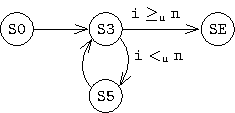
\includegraphics[scale=1.4]{chapters/figures/figMallocSpecCfg.pdf}}
\vspace{15pt}
\end{center}
\caption{\label{fig:llAllocSpecIRCFG}CFG of \SpecL{} program}
\end{subfigure}%
&
\begin{subfigure}[b]{0.5\textwidth}
\begin{center}
{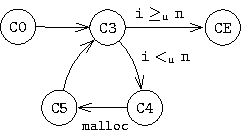
\includegraphics[scale=1.4]{chapters/figures/figMallocCCfg.pdf}}
\end{center}
\caption{\label{fig:llAllocCCFG}CFG of C program}
\end{subfigure}%
\\
\end{tabular}
\caption{\label{fig:mallocSpecCFGAndCCFG}CFG representation of Spec and C IRs shown in \cref{fig:llAllocSpecIR,fig:llAllocCIR} for the {\tt mk\_list} procedures in \cref{fig:llAllocSpec,fig:llAllocC} respectively.}
\end{figure}


Consequently, we are interested in proving that given $\sv{n} = \cv{n}$ at the procedure entries,
$\sv{ret} \indEq{} \lifted{list}{\mem{}}{lnode}{\cv{ret}}$ holds at the exits of both procedures.
Before going into the proof method,
we first introduce an alternate representation of IR, called the Control-Flow Graph (CFG for short).
\Cref{fig:llAllocSpecIRCFG,fig:llAllocCCFG} show the CFG representation of the \SpecL{} and C IRs
in \cref{fig:llAllocSpecIR,fig:llAllocCIR} respectively.
The CFG representation is fundamentally a labeled transition system representation of the corresponding IR,
and is further explored in \cref{sec:ir}.
In essence, each node represents a PC location of its IR, and each edge represents (possibly conditional)
transition between PCs through instruction execution.
For brevity, we often represent a sequence of instructions with a single edge, e.g.,
in \cref{fig:llAllocCCFG}, the edge \cpath{5,3} represents the path \cpath{5,6,7,8,3} in \cref{fig:llAllocCIR}.
\begin{figure}
\begin{tabular}{@{}c@{}c@{}}
\begin{subfigure}[b]{0.5\textwidth}
\begin{center}
{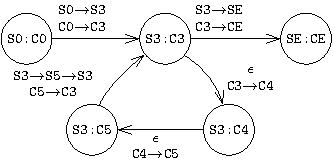
\includegraphics[scale=1.25]{chapters/figures/figMallocProductCfg.pdf}}
\end{center}
\caption{\label{fig:llAllocProductCFG}Product-CFG between CFGs \\ in \cref{fig:llAllocSpecIRCFG,fig:llAllocCCFG}}
\end{subfigure}%
&
\begin{subfigure}[b]{0.5\textwidth}
\begin{center}
\begin{footnotesize}
% \begin{table}
\begin{tabular}{cll}
\toprule
{\bf PC-Pair} & \multicolumn{2}{c}{\bf Invariants} \\
\toprule
(\scpc{0}{0}) & \multicolumn{2}{l}{ $\circled{P}\  \sv{n} = \cv{n}$} \\
\midrule
\multirow{2}{*}{(\scpc{3}{3})} &  $\circled{\scriptsize I1}\  \sv{n} = \cv{n}$ & $\circled{\scriptsize I2}\  \sv{i} = \cv{i}$ \\
&  $\circled{\scriptsize I3}\  \sv{i} \leq_{u} \sv{n}$ & $\circled{\scriptsize I4}\  \sv{l} \indEq{} \lifted{list}{\mem{}}{lnode}{\cv{l}}$ \\
\midrule
(\scpc{3}{4}) &  $\circled{\scriptsize I5}\  \sv{n}=\cv{n}$ & $\circled{\scriptsize I6}\  \sv{i}=\cv{i}$ \\
(\scpc{3}{5}) &  $\circled{\scriptsize I7}\  \sv{i} <_{u} \sv{n}$ & $\circled{\scriptsize I8}\  \sv{l} \indEq{} \lifted{list}{\mem{}}{lnode}{\cv{l}}$ \\
\midrule
(\scpc{E}{E}) & \multicolumn{2}{l}{ $\circled{E}\  \sv{ret} \indEq{} \lifted{list}{\mem{}}{lnode}{\cv{ret}}$} \\
\bottomrule
\end{tabular}
% \end{table}
\end{footnotesize}
\end{center}
\caption{\label{tab:llproductInv}Node invariants for product-CFG in \cref{fig:llAllocProductCFG}}
\end{subfigure}%
\\
\end{tabular}
\caption{\label{fig:llallocProductCFGAndInvs}Product-CFG between the CFGs in \cref{fig:llAllocSpecIRCFG,fig:llAllocCCFG}.
\Cref{tab:llproductInv} contains the corresponding node invariants for the product-CFG.}
\end{figure}

A common approach for showing equivalence between a pair of procedures involves finding a
bisimulation relation across the said procedure-pair.
Intuitively, a bisimulation relation (a) correlates program transitions across the specification
and implementation procedures, and (b) asserts inductively-provable invariants between
machine states of the two procedures at the endpoints of each correlated transition \cite{pnueli98}.
A bisimulation relation itself can be represented as a program, called a {\em product program} \cite{covac}
and its CFG representation is called a {\em product}-CFG.
\Cref{fig:llAllocProductCFG} shows a product-CFG between the \SpecL{} and C {\tt mk\_list} procedures
in \cref{fig:llAllocSpecIRCFG,fig:llAllocCCFG} respectively.

At each node of the product-CFG, {\em invariants} relate the states of the \SpecL{} and C procedures respectively.
\Cref{tab:llproductInv} lists the node invariants for the product-CFG in \cref{fig:llAllocProductCFG}.
At the start node (\scpc{0}{0}) of the product-CFG, the precondition (labeled \circled{\small P})
ensures equality of input arguments \sv{n} and \cv{n} at the procedure entries.
Inductive invariants (labeled \circled{I}) need to be inferred at
each intermediate product-CFG node (e.g., (\scpc{3}{3})) relating both programs' states.
For example, at node (\scpc{3}{5}), \circled{\small I6} $\sv{i} = \cv{i}$ is an inductive invariant.
The inductive invariant \circled{\small I4} $\sv{l} \indEq{} \lifted{list}{\mem{}}{lnode}{\cv{l}}$
is another example of a \recursiveRelation{} and asserts equality between the intermediate \SpecL{} and C lists
at their respective loop heads.
Assuming that the precondition (\circled{\small P}) holds at the entry node (\scpc{0}{0}),
a bisimulation check involves checking that the inductive invariants hold too,
and consequently the postcondition (\circled{\small E}) holds at the exit node (\scpc{E}{E}).
Checking correctness of a bisimulation relation involves checking whether an invariant holds (among other things).
These checks result in proof queries which must be discharged by a solver (aka theorem prover).

\section{Our Contributions}
\label{sec:contribs}
As previously summarized in \cref{sec:motivatingexample}, an algorithm to find a bisimulation based proof of equivalence
between a \SpecL{} and C procedure involves three major algorithms:
\curved{A1} An algorithm for construction of a product-CFG by correlating program executions
across the \SpecL{} and C procedures respectively.
\curved{A2} An algorithm for identification of inductively-provable invariants at intermediate correlated PCs.
\curved{A3} An algorithm for solving proof obligations generated by \curved{A1} and \curved{A2} algorithms.
Next we list our major contributions.

\subsection*{Proof Discharge Algorithm}
Solving proof obligations (\curved{A3}) involving \recursiveRelations{}
(generated by \curved{A1} and \curved{A2}) is quite interesting and forms our primary contribution.
We describe a {\em sound} proof discharge algorithm capable of tackling proof obligations containing
\recursiveRelations{} using off-the-shelf SMT solvers. Our proof discharge algorithm is also capable of
reconstruction of counterexamples for the original proof query from models returned by the individual SMT queries.
These counterexamples form the foundation of counterexample-guided heuristics for \curved{A1} and \curved{A2} algorithms
as we will discuss shortly.
As part of our proof discharge algorithm,
we reformulate equality of ADT values (i.e. \recursiveRelations{}) as equivalence of programs
and discharge these proof queries using a nested (albeit much simpler) equivalence check.

\subsection*{Spec-to-C Automatic Equivalence Checker Tool}
Our second contribution is \toolName{}, a {\em sound} equivalence checker tool
capable of proving equivalence between a \SpecL{} and a C program automatically.
\toolName{} either successfully finds a bisimulation relation implying equivalence or it provides a (sound but incomplete) unknown verdict.
\toolName{} builds upon the Counter tool\cite{oopsla20} and uses specialized versions of (a) counterexample-guided correlation algorithm for
incremental construction of a product-CFG (\curved{A1}) and (b) counterexample-guided invariant inference algorithm
for inference of inductive invariants at correlated PCs in the (partially constructed) product-CFG (\curved{A2})
based on prior work on counterexample-guided equivalence checking \cite{shubhanipdhthesis}.
\toolName{} discharges the required verification conditions (i.e. proof obligations) using our Proof Discharge Algorithm.
The counterexamples generated by the proof discharge algorithm help steer the search algorithms \curved{A1} and \curved{A2}.

\section{Outline of the Thesis}
\label{sec:outline}
The rest of the thesis is divided into five chapters.
We begin with a thorough presentation of the topics introduced thus far in \cref{sec:prelims}.
The major topics discussed include our specification language, logical representation of programs, and bisimulation
in the context of \SpecL{}-C equivalence.
We finish \cref{sec:prelims} with a logical encoding of proof obligations generated during an equivalence check.

The next chapter, \cref{sec:examples} illustrates our proof discharge algorithm (\curved{A3}) through
proof obligations originating from equivalence checks between previously shown program-pairs.
In the context of our proof discharge algorithm, we introduce a decomposition procedure based on unification
to reduce a \recursiveRelation{} to an equivalent set of equalities.
The proof discharge algorithm categorizes a proof obligation into three types, each of which is
illustrated with the help of examples.
We finish with a summary and pseudocode of the algorithm.

\Cref{sec:spectocalgo} gives an exhaustive overview of the major components of our Spec-to-C equivalence checker tool, \toolName{}.
We begin with a dataflow formulation of the points-to analysis introduced as part of our proof discharge algorithm in \cref{sec:examples}.
Next, we summarize the counterexample driven algorithms for product-CFG construction (\curved{A1})
and invariant inference (\curved{A2}) based on prior work \cite{shubhanipdhthesis}.
\Cref{sec:spectocalgo} presents the pseudocode for the major subprocedures used as part of our
proof discharge algorithm, in addition to details of SMT encoding of proof obligations and
recovery of counterexamples from SMT models.
We finish with a new representation of expressions, called `Value Trees' which enables the consolidation
of multiple subprocedures utilized as a component of our proof discharge algorithm.
We also present an algorithm for converting an expression to its value tree representation
along with illustrative examples of its applications.

We provide a comprehensive evaluation of \toolName{} in \cref{sec:eval}, followed by its limitations.
\Cref{sec:conclusion} concludes our work by reiterating the key ideas presented, alongside additional related work.
